\section{Results}


LUX's NEST simulations closely predicted the electron recoil band.  In the first ?? hours of data there were ?? $\pm$ ?? events inside of the predicted ER band out of a total of ?? $\pm$ ?? events in the fiducial region.  Thus, the 90\% confidence bands constructed by NEST contained ??\% $\pm$ ??\% of the tritium events.  

NOTE: MAKE NEST PLOTS FOR FID

The mass of xenon in the fiducial volume is 125 kg, while the entire mass of liquid xenon seen by the PMTs is 285 kg.  The total number of tritium events seen in the first ?? hours within the fiducial volume is ?? $\pm$ ??, while the total number of tritium events seen in the first ?? hours in the entire detector is ?? $\pm$ 32.4.  Since the event ratio in the fiducial volume compared to the total volume is ?? $\pm$ ??, and the mass ratio of the fiducial volume to the total volume is ??, the tritium events appear to be fairly uniform throughout the detector.

The event rate in the LUX detector returned to the initial background rate of ?? $\pm$ ?? Hz after ?? days.  A comparison of events in the fiducial region before and after the CH$_3$T calibration shows the complete removal of the CH$_3$T source.

\begin{figure}[h]
\centering
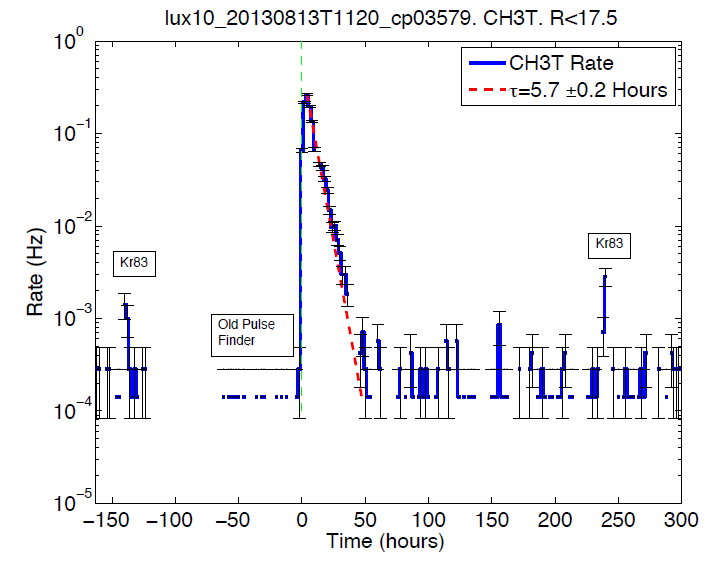
\includegraphics[scale=0.25]{LUXTimeHisto.png}
\caption{A time histogram of the ?? Bq CH$_3$T injection into LUX.}
\label{fig:TimeHisto}
\end{figure}

\begin{figure}[h]
\centering
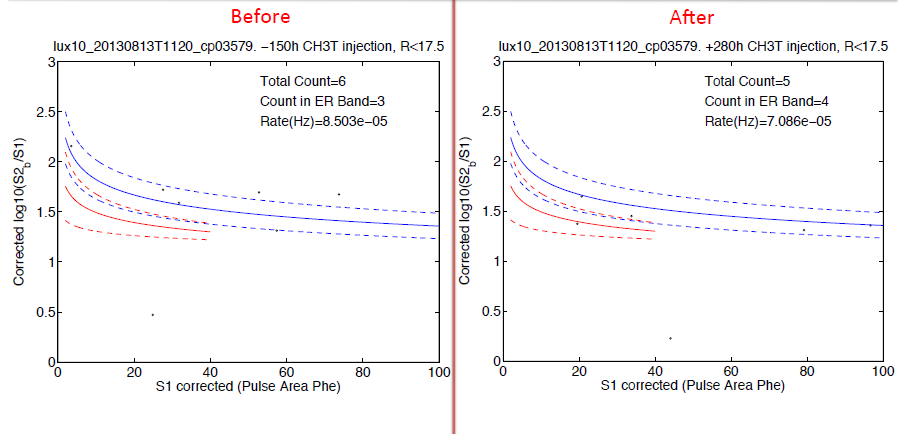
\includegraphics[scale=0.25]{BeforeAndAfter.png}
\caption{Events in the fiducial region of LUX before and after the CH$_3$T calibration.}
\label{fig:BandA}
\end{figure}


NOTE: MAKE DISTRIBUTION AND SPREAD PLOTS 
NOTE: MAKE PLOTS AND REDO NUMBERS AFTER DATA HAS BEEN REPROCESSED